
%%%%%%%%%%%%%%%%%%%%%%%%%%%%%%%%%%%%%%%%%%%%%%%%%%%%%%%%%%%%%%%%%%%%%%%%%%%%%%%%%%
\begin{frame}[fragile]\frametitle{}
\begin{center}
{\Large Limits}
\end{center}
\end{frame}

%%%%%%%%%%%%%%%%%%%%%%%%%%%%%%%%%%%%%%%%%%%%%%%%%%%%%%%%%%%
 \begin{frame}[fragile]\frametitle{Limits}
\begin{itemize}
\item Functions can be plotted, with input(s) on say x and output on y (higher dimension functions, not considered as of now)
\item Say, $f(x) = x + 2$ is function showing distance traveled (y) at each x seconds.
\item Slope gives rate of change, ie Speed.and its constant.
\item It can be calculated by taking any two points on the line
\end{itemize}
\begin{center}
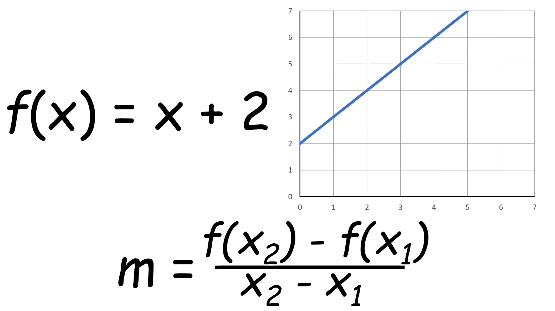
\includegraphics[width=0.5\linewidth,keepaspectratio]{func4}
\end{center}
\end{frame}

%%%%%%%%%%%%%%%%%%%%%%%%%%%%%%%%%%%%%%%%%%%%%%%%%%%%%%%%%%%
 \begin{frame}[fragile]\frametitle{Exercise}
$q(x) = 2x+1$

\begin{lstlisting}
def q(x):
    return 2*x + 1

import numpy as np
from matplotlib import pyplot as plt

x = np.array(range(0, 11))

plt.xlabel('Seconds')
plt.ylabel('Meters')
plt.xticks(range(0,11, 1))
plt.yticks(range(0, 22, 1))
plt.grid()

plt.plot(x,q(x), color='green')
plt.show()
\end{lstlisting}
\end{frame}


%%%%%%%%%%%%%%%%%%%%%%%%%%%%%%%%%%%%%%%%%%%%%%%%%%%%%%%%%%%
 \begin{frame}[fragile]\frametitle{Plot}
\begin{center}
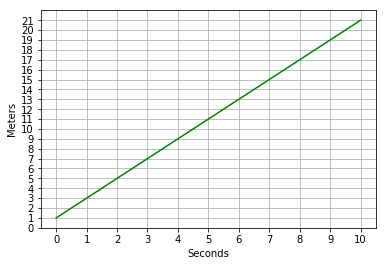
\includegraphics[width=0.7\linewidth,keepaspectratio]{func6}
\end{center}
\end{frame}

%%%%%%%%%%%%%%%%%%%%%%%%%%%%%%%%%%%%%%%%%%%%%%%%%%%%%%%%%%%
 \begin{frame}[fragile]\frametitle{Functions}
\begin{itemize}
\item If $f(x) = x^2 + 1$ is function showing distance traveled (y) at each x seconds.
\item Secant Slope gives rate of change, ie Speed. and its approximate.
\item For different secants, different slopes, so any change in speed is called acceleration.
\end{itemize}
\begin{center}
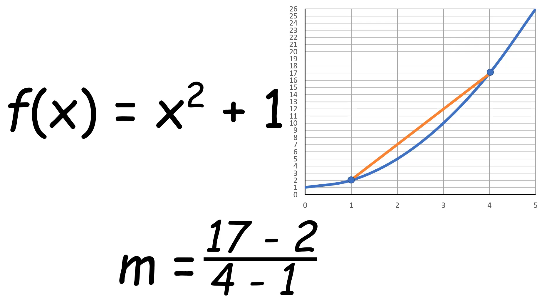
\includegraphics[width=0.5\linewidth,keepaspectratio]{func5}
\end{center}
\end{frame}


%%%%%%%%%%%%%%%%%%%%%%%%%%%%%%%%%%%%%%%%%%%%%%%%%%%%%%%%%%%
 \begin{frame}[fragile]\frametitle{Exercise}
$r(x) = x^2 + x$

\begin{lstlisting}
def r(x):
    return x**2 + x

import numpy as np
from matplotlib import pyplot as plt

# Create an array of x values from 0 to 10
x = np.array(range(0, 11))

# Create an array for the secant line
s = np.array([0,10])

plt.xlabel('Seconds')
plt.ylabel('Meters')
plt.grid()

# Plot x against r(x)
plt.plot(x,r(x), color='green')

# Plot the secant line
plt.plot(s,r(s), color='magenta')
plt.show()
\end{lstlisting}
\end{frame}


%%%%%%%%%%%%%%%%%%%%%%%%%%%%%%%%%%%%%%%%%%%%%%%%%%%%%%%%%%%
 \begin{frame}[fragile]\frametitle{Plot}
\begin{center}
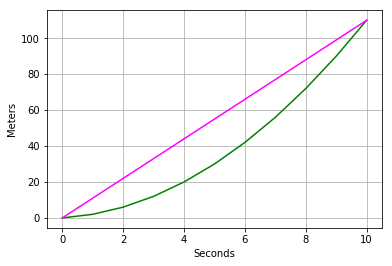
\includegraphics[width=0.7\linewidth,keepaspectratio]{func7}
\end{center}
Average velocity is 10 m/s
\end{frame}

%%%%%%%%%%%%%%%%%%%%%%%%%%%%%%%%%%%%%%%%%%%%%%%%%%%%%%%%%%%
 \begin{frame}[fragile]\frametitle{Practical Example}
\begin{itemize}
\item Say, Pune (P), and Mumbai (M) are 200km apart.
\item It takes 4hrs to cover the distance, so the average velocity is $\frac{200}{4} = 50kmph$.
\item Is that the velocity throughout the journey?
\item At Wakad, it could be 20, highway it could be 100, etc.
\item Within Lonawala, which is about 1km wide, whats the average velocity? you can measure from start, end of 1km, and decide.
\item What's the velocity while crossing Maganlal shop? which is about 10m long?
\item We are narrowing down, to find what is called `instantaneous' velocity.
\item Very small, infinitesimally small, a point.
\item Limiting condition.
\end{itemize}
\end{frame}


%%%%%%%%%%%%%%%%%%%%%%%%%%%%%%%%%%%%%%%%%%%%%%%%%%%%%%%%%%%
 \begin{frame}[fragile]\frametitle{Instantaneous Velocity?}
\begin{itemize}
\item Secant is an approximation, not an exact speed at a particular moment.
\item We need slope of a curve AT A SINGLE POINT (and not approximate average between two secant points)
\item If we want slope at a particular x, we can find slope of a secant between x1 and x2 which are very close to x.
\end{itemize}
\end{frame}

%%%%%%%%%%%%%%%%%%%%%%%%%%%%%%%%%%%%%%%%%%%%%%%%%%%%%%%%%%%
 \begin{frame}[fragile]\frametitle{Instantaneous Velocity?}
\begin{itemize}
\item For a point on the curve ,say, (3,10)
\item From left and right sides we can approxa the point.
\item Y values at such nearby points is called as LIMIT
\end{itemize}
\begin{center}
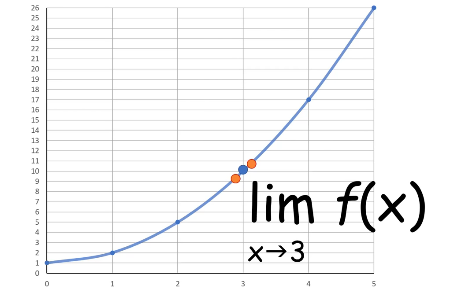
\includegraphics[width=0.5\linewidth,keepaspectratio]{func8}
\end{center}
\end{frame}


%%%%%%%%%%%%%%%%%%%%%%%%%%%%%%%%%%%%%%%%%%%%%%%%%%%%%%%%%%%
 \begin{frame}[fragile]\frametitle{Continuity}
\begin{itemize}
\item Most functions we looked at so far, are continuous for all real values of $x$
\item Meaning if you trace them, you need not lift your pen.
\item Not all functions are defined like that.
\item $f(x) = \frac{x^2}{x+1}, x \leq -2 | x \geq 0$
\item Obviously, there is a gap in the domain as well as output, so not continuous.
\end{itemize}
\begin{center}
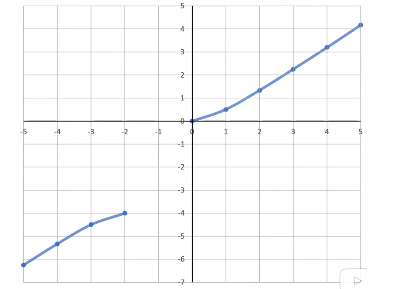
\includegraphics[width=0.5\linewidth,keepaspectratio]{func9}
\end{center}
\end{frame}

%%%%%%%%%%%%%%%%%%%%%%%%%%%%%%%%%%%%%%%%%%%%%%%%%%%%%%%%%%%
 \begin{frame}[fragile]\frametitle{Finding Limits}
 What is meant by finding limits of a function at a particular x?
\begin{itemize}
\item Go from left side (ie less of x, increasing) and see to which value $f(x)$ is approaching.
\item Go from right side (ie more of x, decreasing) and see to which value $f(x)$ is approaching.
\item If both results are same, we got the limit value.
\item Even if $f(x)$ is not defined for that x, the limit value exists!!!
\end{itemize}
\begin{center}
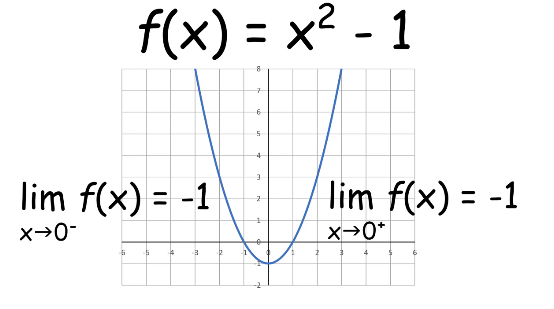
\includegraphics[width=0.5\linewidth,keepaspectratio]{func10}
\end{center}
\end{frame}

%%%%%%%%%%%%%%%%%%%%%%%%%%%%%%%%%%%%%%%%%%%%%%%%%%%%%%%%%%%
 \begin{frame}[fragile]\frametitle{Finding Limits}
\begin{itemize}
\item Lets look at obvious non continuous function
\item Need to find limit of function at x = -1
\item From negative side, the $f(x)$ is projected to go to 3.7 or so for x = -1
\item From positive side, the $f(x)$ is projected to go to -0.3 so for x = -1
\item Both do NOT agree. So limit does not exists.
\end{itemize}
\begin{center}
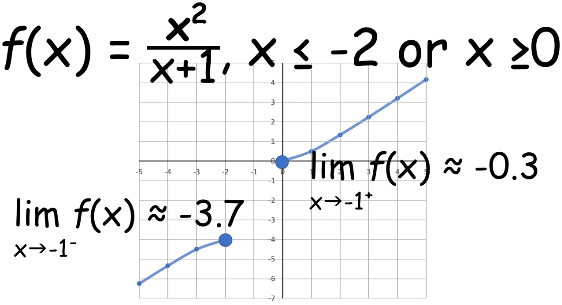
\includegraphics[width=0.5\linewidth,keepaspectratio]{func11}
\end{center}
\end{frame}


%%%%%%%%%%%%%%%%%%%%%%%%%%%%%%%%%%%%%%%%%%%%%%%%%%%%%%%%%%%
 \begin{frame}[fragile]\frametitle{Finding Limits}
\begin{itemize}
\item Lets look at single point non continuous function
\item Need to find limit of function at x = 0
\item Calculate values from both sides
\item The limit is approaching to 2
\end{itemize}
\begin{center}
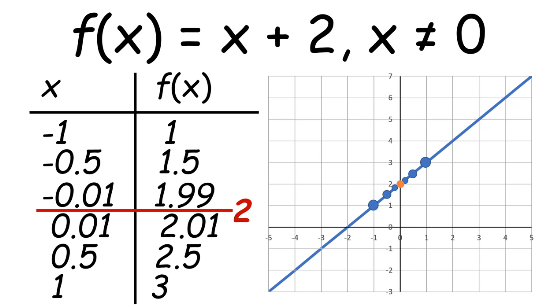
\includegraphics[width=0.5\linewidth,keepaspectratio]{func12}
\end{center}
Why not just substitute the value?
\end{frame}



%%%%%%%%%%%%%%%%%%%%%%%%%%%%%%%%%%%%%%%%%%%%%%%%%%%%%%%%%%%
 \begin{frame}[fragile]\frametitle{Exercise}
$g(x) = -(\frac{12}{2x})^2, x \neq 0$

\begin{lstlisting}
def g(x):
    if x != 0:
        return -(12/(2*x))**2
    
from matplotlib import pyplot as plt

x = range(-20, 21)
y = [g(a) for a in x]

plt.xlabel('x')
plt.ylabel('g(x)')
plt.grid()

# Plot x against g(x)
plt.plot(x,y, color='green')

plt.show()
\end{lstlisting}
\end{frame}

%%%%%%%%%%%%%%%%%%%%%%%%%%%%%%%%%%%%%%%%%%%%%%%%%%%%%%%%%%%
 \begin{frame}[fragile]\frametitle{Plot}
\begin{center}
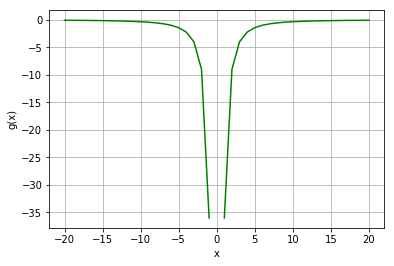
\includegraphics[width=0.6\linewidth,keepaspectratio]{func13}
\end{center}

\end{frame}


%%%%%%%%%%%%%%%%%%%%%%%%%%%%%%%%%%%%%%%%%%%%%%%%%%%%%%%%%%%
 \begin{frame}[fragile]\frametitle{Exercise}
$d(x) = \frac{4}{x-25}, x \neq 25$

\begin{lstlisting}
def d(x):
    if x != 25:
        return 4 / (x - 25)

from matplotlib import pyplot as plt
x = list(range(-100, 24))
x.append(24.9) # Add some fractional x
x.append(25)   # values around
x.append(25.1) # 25 for finer-grain results
x = x + list(range(26, 101))
# Get the corresponding y values from the function
y = [d(i) for i in x]

plt.xlabel('x')
plt.ylabel('d(x)')
plt.grid()

plt.plot(x,y, color='purple')
plt.show()
\end{lstlisting}
\end{frame}

%%%%%%%%%%%%%%%%%%%%%%%%%%%%%%%%%%%%%%%%%%%%%%%%%%%%%%%%%%%
 \begin{frame}[fragile]\frametitle{Plot}
\begin{center}
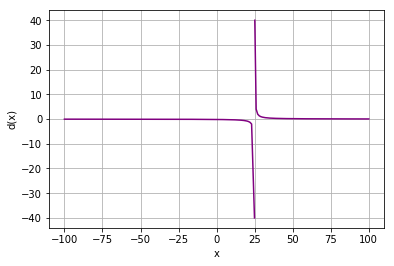
\includegraphics[width=0.5\linewidth,keepaspectratio]{func14}
\end{center}
If we were to plot every fractional value of d(x) for x values between 24.9 and 25, we'd see a line that decreases indefinitely, getting closer and closer to the $x = 25$ vertical line, but never actually reaching it. Similarly, plotting every x value between 25 and 25.1 would result in a line going up indefinitely, but always staying to the right of the vertical $x = 25$ line.
\end{frame}

%%%%%%%%%%%%%%%%%%%%%%%%%%%%%%%%%%%%%%%%%%%%%%%%%%%%%%%%%%%
 \begin{frame}[fragile]\frametitle{Plot}
\begin{center}
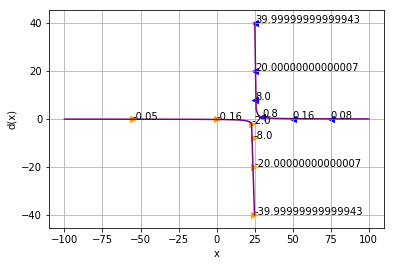
\includegraphics[width=0.5\linewidth,keepaspectratio]{func15}
\end{center}
The $x = 25$ line in this case is an asymptote - a line to which a curve moves ever closer but never actually reaches. The positive limit for $x = 25$ in this case in not a real numbered value, but infinity:

$\lim_{x \to 25+} d(x) = \infty$

$\lim_{x \to 25-} d(x) = \infty$
\end{frame}



%%%%%%%%%%%%%%%%%%%%%%%%%%%%%%%%%%%%%%%%%%%%%%%%%%%%%%%%%%%
 \begin{frame}[fragile]\frametitle{Finding Limits}
Direct Substitution
$g(x) = \frac{x^2 - 1}{x - 1}, x \neq 1$
\begin{center}
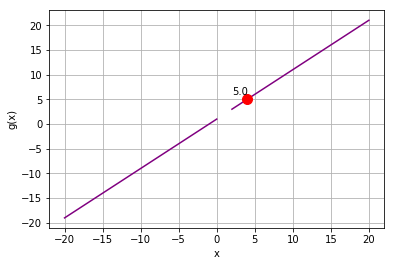
\includegraphics[width=0.5\linewidth,keepaspectratio]{func16}
\end{center}
Find the limit of g(x) as x approaches 4. Just substitute and get the limit as 5.
\end{frame}

%%%%%%%%%%%%%%%%%%%%%%%%%%%%%%%%%%%%%%%%%%%%%%%%%%%%%%%%%%%
 \begin{frame}[fragile]\frametitle{Finding Limits}
Factorization
$g(x) = \frac{x^2 - 1}{x - 1}, x \neq 1$
\begin{center}
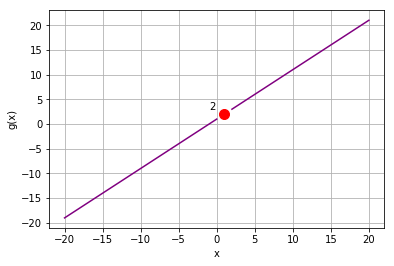
\includegraphics[width=0.5\linewidth,keepaspectratio]{func17}
\end{center}
Find the limit of g(x) as x approaches 1. Substituting gives 0/0, so not good. Factorize and cancel common portion $(x -1)$. Then substitute. Result is 2.
\end{frame}

%%%%%%%%%%%%%%%%%%%%%%%%%%%%%%%%%%%%%%%%%%%%%%%%%%%%%%%%%%%
 \begin{frame}[fragile]\frametitle{Finding Limits}
Rationalization
$h(x) = \frac{\sqrt x - 2}{x - 4}, x \neq 4 and x \geq 0$
\begin{center}
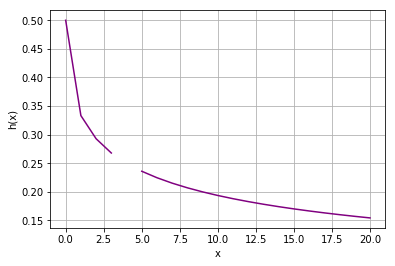
\includegraphics[width=0.5\linewidth,keepaspectratio]{func18}
\end{center}
Multiply top and bottom by $\sqrt x + 2$. Then substitute x = 4.. Result is 0.25
\end{frame}


%%%%%%%%%%%%%%%%%%%%%%%%%%%%%%%%%%%%%%%%%%%%%%%%%%%%%%%%%%%
 \begin{frame}[fragile]\frametitle{Rules of Limits}
\begin{itemize}
\item $\lim_{x \to a} (j(x) + l(x)) = \lim_{x \to a} j(x) + \lim_{x \to a} l(x)$
\item $\lim_{x \to a} (j(x) - l(x)) = \lim_{x \to a} j(x) - \lim_{x \to a} l(x)$
\item $\lim_{x \to a} (j(x) \cdot l(x)) = \lim_{x \to a} j(x) \cdot \lim_{x \to a} l(x)$
\item $\lim_{x \to a} \frac{j(x)}{l(x)} = \frac{\lim_{x \to a} j(x)}{\lim_{x \to a} l(x)}$
\item $\lim_{x \to a} (j(x))^{n} = \Big(\lim_{x \to a} j(x)\Big)^{n}$
\end{itemize}

\end{frame}




%%%%%%%%%%%%%%%%%%%%%%%%%%%%%%%%%%%%%%%%%%%%%%%%%%%%%%%%%%%
\begin{frame}[fragile]\frametitle{}
 
\textbf{Example}
Consider the function $f(x,y)= \frac{\sin(x^2+y^2)}{x^2+y^2}$ near $(0,0)$.

\ \\  \ \\
\begin{tabular}{|c|c|c|c|c|c|c|c|}
\hline
$x\backslash y$&-1.000&-0.667&-0.333&0.000&0.333&0.667&1.000 \\ 
\hline
-1.000&0.455&0.687&0.807&0.841&0.807&0.687&0.455\\ 
\hline
-0.667&0.687&0.873&0.949&0.967&0.949&0.873&0.687\\ 
\hline
-0.333&0.807&0.949&0.992&0.998&0.992&0.949&0.807\\ 
\hline
0.000&0.841&0.967&0.998& - &0.998&0.967&0.841\\ 
\hline
0.333&0.807&0.949&0.992&0.998&0.992&0.949&0.807\\ 
\hline
0.667&0.687&0.873&0.949&0.967&0.949&0.873&0.687\\ 
\hline
1.000&0.455&0.687&0.807&0.841&0.807&0.687&0.455\\ 
\hline
\end{tabular} 
\  \\ \ \\
It seems reasonable to say that $\lim_{(x,y) \rightarrow (0,0)} f(x,y)=1$.


\end{frame}


%%%%%%%%%%%%%%%%%%%%%%%%%%%%%%%%%%%%%%%%%%%%%%%%%%%%%%%%%%%
\begin{frame}[fragile]\frametitle{}
 
\textbf{Example}
Consider the function $g(x,y) = \frac{ (x^2-y^2)^2 }{(x^2+y^2)^2}$.  
\ \\ \ \\
\begin{tabular}{|c|c|c|c|c|c|c|c|}
\hline
$x\backslash y$&-1.000&-0.667&-0.333&-0.000&0.333&0.667&1.000 \\ 
\hline
-1.000&0.000&0.148&0.640&1.000&0.640&0.148&0.000\\ 
\hline
-0.667&0.148&0.000&0.360&1.000&0.360&0.000&0.148\\ 
\hline
-0.333&0.640&0.360&0.000&1.000&0.000&0.360&0.640\\ 
\hline
-0.000&1.000&1.000&1.000& - &1.000&1.000&1.000\\ 
\hline
0.333&0.640&0.360&0.000&1.000&0.000&0.360&0.640\\ 
\hline
0.667&0.148&0.000&0.360&1.000&0.360&0.000&0.148\\ 
\hline
1.000&0.000&0.148&0.640&1.000&0.640&0.148&0.000\\ 
\hline
\end{tabular}  
\ \\ \ \\
Here we say that $\lim_{(x,y) \rightarrow (0,0)} g(x,y)$ does not exist.  \\ 
For a better understanding of the problem try approaching $(0,0)$ along the line $y=mx$.


\end{frame}


%%%%%%%%%%%%%%%%%%%%%%%%%%%%%%%%%%%%%%%%%%%%%%%%%%%%%%%%%%%
\begin{frame}[fragile]\frametitle{}
 
\textbf{Definition}
Suppose that $f(x,y)$ has domain $D$ and that $(a,b)$ is in the interior of $D$.  Then we say that the \underline{limit of $f(x,y)$ as
$(x,y)$} \underline{approaches $(a,b)$} is $L$ and write
$$
\lim_{(x,y)\rightarrow (a,b)} f(x,y) = L,
$$
if for every $\epsilon >0$ there is a corresponding number $\delta>0$ such that if $(x,y)\in D$ and if $|(x,y),(a,b)|<\delta$, then
$|f(x,y)-L|<\epsilon$.
  

\textbf{Note}
Suppose that $f(x,y)$ is a function of two variables and that $C_1$ and $C_2$ are two curves which intersect at $(a,b)$.  If $f(x,y)\rightarrow L_1$ as $(x,y)\rightarrow (a,b)$ along $C_1$ and $f(x,y)\rightarrow L_2$ as $(x,y)\rightarrow (a,b)$ along $C_2$ and if $L_1\neq L_2$ then $\lim_{(x,y)\rightarrow (a,b)} f(x,y)$ does not exist.

\end{frame}



%%%%%%%%%%%%%%%%%%%%%%%%%%%%%%%%%%%%%%%%%%%%%%%%%%%%%%%%%%%
\begin{frame}[fragile]\frametitle{}
 
\textbf{Example}
Consider the function $f(x,y)=\frac{xy^2}{x^2+y^4}$.  Does $\lim_{(x,y)\rightarrow (0,0} f(x,y)$ exit?
 

\textbf{Example}
Consider the function $f(x,y)=\frac{x^2y}{x^2+y^2}$.  Compute $\lim_{(x,y)\rightarrow (0,0} f(x,y)$.
 

\textbf{Note} 
\begin{enumerate}
\item $\lim_{(x,y)\rightarrow (a,b)} x = a$,  $\lim_{(x,y)\rightarrow (a,b)} y = b$, $\lim_{(x,y)\rightarrow (a,b)} c = c$.  
\item $\lim_{(x,y)\rightarrow (a,b)} (f(x,y)+g(x,y)) = \lim_{(x,y)\rightarrow (a,b)} f(x,y) + \lim_{(x,y)\rightarrow (a,b)} g(x,y)$. 
\item $\lim_{(x,y)\rightarrow (a,b)} f(x,y)g(x,y) = \lim_{(x,y)\rightarrow (a,b)} f(x,y) \cdot \lim_{(x,y)\rightarrow (a,b)} g(x,y)$. 
\item $\lim_{(x,y)\rightarrow (a,b)} \frac{f(x,y)}{g(x,y)} = \frac{\lim_{(x,y)\rightarrow (a,b)} f(x,y)}{\lim_{(x,y)\rightarrow (a,b)} g(x,y)}$.
\end{enumerate}

\end{frame}



%%%%%%%%%%%%%%%%%%%%%%%%%%%%%%%%%%%%%%%%%%%%%%%%%%%%%%%%%%%
\begin{frame}[fragile]\frametitle{}
 
\textbf{Definition}
We say that $f(x,y)$ is \underline{continuous at $(a,b)$} if 
$$
\lim_{(x,y)\rightarrow (a,b)} f(x,y) = f(a,b).
$$  
We say that $f$ is \underline{continuous on $D$} is $f$ is continuous at each point of $D$.
  

\textbf{Note}
Using properties of limits, one can prove that if $f$ and $g$ are continuous on their domains then so are $f+g$, $f-g$, $fg$ and $f/g$.  Note that any zeros of $g$ will not be in the domain of $f/g$.
 

\textbf{Fact}
Polynomials and rational functions (ratios of polynomials) are continuous on their domain.

\end{frame}



%%%%%%%%%%%%%%%%%%%%%%%%%%%%%%%%%%%%%%%%%%%%%%%%%%%%%%%%%%%
\begin{frame}[fragile]\frametitle{}
 
\textbf{Example}
\begin{enumerate}
\item  Consider the function $g(x,y) = \frac{ (x^2-y^2)^2 }{(x^2+y^2)^2}$.  Where is $g$ continuous?  
\item  What about the function 
                $$h(x,y)=\begin{cases}
                                     \frac{ (x^2-y^2)^2 }{(x^2+y^2)^2} & \mbox{if $(x,y)\neq (0,0)$}, \\
                                      0  & \mbox{if $(x,y)=(0,0)$}?
                                \end{cases}
                 $$
\item  Where is the function 
                  $$f(x,y)=\begin{cases}
                                      \frac{x^2y}{x^2+y^2} & \mbox{if $(x,y)\neq (0,0)$}, \\
                                      0  & \mbox{if $(x,y)=(0,0)$}.
                                \end{cases}
                 $$
           continuous?
\end{enumerate}

\end{frame}


%%%%%%%%%%%%%%%%%%%%%%%%%%%%%%%%%%%%%%%%%%%%%%%%%%%%%%%%%%%
\begin{frame}[fragile]\frametitle{}
 
\textbf{Fact}
Suppose that $f(x,y)$ and $g(t)$ are continuous functions with $g$ defined on the range of $f$.  Then $g\circ f$ is continuous on the domain of $f$.
  

\textbf{Example}
\begin{enumerate}
\item  Where is the function $h(x,y)=|(x,y)|$ continuous?  
\item  Where is the function $\sin(y/x)$ continuous?
\end{enumerate}

\end{frame}

%%%%%%%%%%%%%%%%%%%%%%%%%%%%%%%%%%%%%%%%%%%%%%%%%%%%%%%%%%%
\begin{frame}[fragile] \frametitle{Functions of 3 or more variables}
\textbf{Definition}
If $f$ is a real valued function defined on $D\subseteq \mathbb R^n$, then we say that $\lim_{\vec{x}\rightarrow\vec{a}} f(\vec{x})=L$ if
for all $\epsilon >0$, there is $\delta > 0$ such that whenever $|\vec{x}-\vec{a}|<\delta$, $|f(\vec{x})-L|<\epsilon$, where 
$|\vec{x}-\vec{a}| =\sqrt{(x_1-a_1)^2 +\dots +(x_n-a_n)^2}$.
  

\textbf{Definition}
Suppose that $f$ is a real valued function defined on $D\subseteq \mathbb R^n$.  Then we say that $f$ is continuous at $\vec{a}\in \mathbb R^n$ if
$$
\lim_{\vec{x}\rightarrow\vec{a}} f(\vec{x}) =f(\vec{a}).
$$

\end{frame}
